The Neutrino Experiment with a Xenon TPC (NEXT) \cite{NEXT:2011eyk} will search for \bbonu\ in \XE\ using a 100-kg high-pressure gaseous xenon (HPXe) time projection chamber. 
Such a detector can provide both good energy resolution and event topological information for background rejection \cite{Nygren:2009zz}.

Double beta decay events leave a distinctive topological signature in HPXe: a ionization track, of about 30 cm long at 10 bar, tortuous due to multiple scattering, and with larger energy depositions at both ends (see fig.~\ref{fig:next_track}). The Gotthard experiment \cite{Luscher:1998sd}, consisting in a small xenon TPC (5.3 kg of xenon, 68\% enrichment in \XE ) operated at 5 bar, proved the effectiveness of such a signature to reject background, achieving a background rate of only $\sim0.01$ \ckky.

%%%%%
\begin{figure}[t!]
\vspace{0.75cm}
\begin{center}
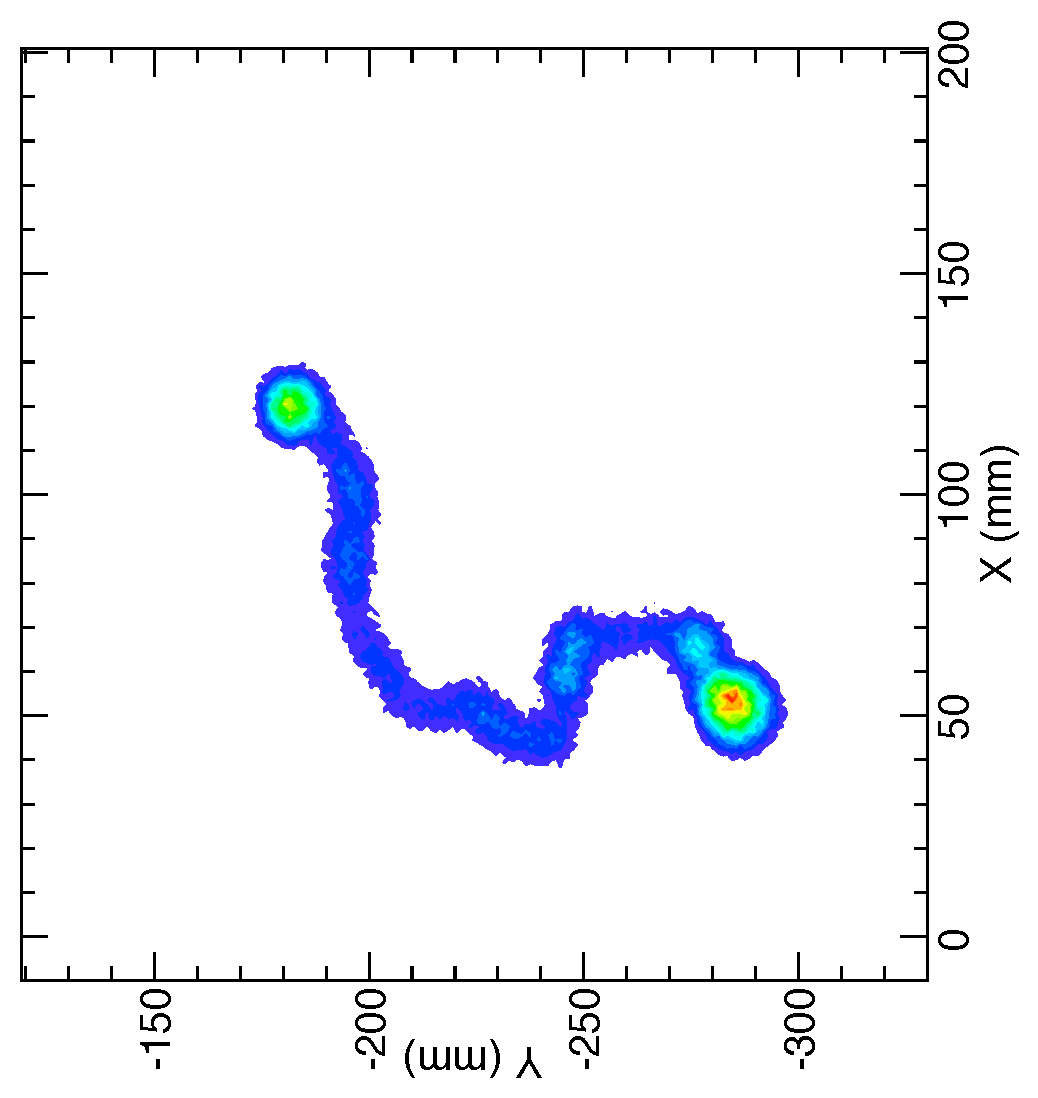
\includegraphics[angle=-90,scale=0.45]{img/bb0nu_track_10atm.eps}
\end{center}
\caption{Simulation of a \bbonu\ track in gaseous xenon at 10 bar \cite{NEXT:2011eyk}.} \label{fig:next_track}
\end{figure}
%%%%%

The design of NEXT is optimized for energy resolution (better than 1\% FWHM at $Q_{\beta \beta}$) by using proportional electroluminescent (EL) amplification of the ionization signal. The detection process is as follows. Particles interacting in the HPXe transfer their energy to the medium through ionization and excitation. The excitation energy is manifested in the prompt emission of VUV ($\sim$178 nm) scintillation light. The ionization tracks (positive ions and free electrons) left behind by the particle are prevented from recombination by a strong electric field (0.5--1.0 kV/cm). Negative charge carriers drift toward the TPC anode, entering a region, defined by two highly-transparent meshes, with an even more intense electric field (3.5 kV/cm/bar). There, further VUV photons are generated isotropically by electroluminescence. Therefore, both scintillation and ionization produce an optical signal, to be detected with a sparse plane of PMTs located behind the cathode. The detection of the primary scintillation light constitutes the start-of-event ($t_0$), whereas the detection of EL light provides an energy measurement. Electroluminescent light provides tracking as well, since it is detected also a few mm away from production at the anode plane, via a dense array (1 cm pitch) of 1-mm$^{2}$ SiPMs.

The NEXT detector will operate at 10 bar, with xenon enriched at 90\% in the \XE\ isotope. At that pressure the 100 kg mass of xenon results in a volume of $\sim$2.5 m$^3$.

The major benefits of the NEXT 100 proposal are its high background rejection factor, resulting in an expected background rate of $2\times 10^{-4}$ \ckkbby , and the fact that xenon is relatively easy (cheap) to enrich and obtain in large quantities.

The NEXT Collaboration expects to commission the detector at the end of 2013. The experiment plans to start its physics run in the second half of 2014.
